% Options for packages loaded elsewhere
\PassOptionsToPackage{unicode}{hyperref}
\PassOptionsToPackage{hyphens}{url}
\PassOptionsToPackage{dvipsnames,svgnames,x11names}{xcolor}
%
\documentclass[
]{article}

\usepackage{amsmath,amssymb}
\usepackage{iftex}
\ifPDFTeX
  \usepackage[T1]{fontenc}
  \usepackage[utf8]{inputenc}
  \usepackage{textcomp} % provide euro and other symbols
\else % if luatex or xetex
  \usepackage{unicode-math}
  \defaultfontfeatures{Scale=MatchLowercase}
  \defaultfontfeatures[\rmfamily]{Ligatures=TeX,Scale=1}
\fi
\usepackage{lmodern}
\ifPDFTeX\else  
    % xetex/luatex font selection
    \setmainfont[]{TeX Gyre Pagella}
    \setsansfont[]{TeX Gyre Heros}
  \setmathfont[]{Asana Math}
\fi
% Use upquote if available, for straight quotes in verbatim environments
\IfFileExists{upquote.sty}{\usepackage{upquote}}{}
\IfFileExists{microtype.sty}{% use microtype if available
  \usepackage[]{microtype}
  \UseMicrotypeSet[protrusion]{basicmath} % disable protrusion for tt fonts
}{}
\usepackage{xcolor}
\usepackage[top=10pc,bottom=10pc,left=11pc,right=11pc,heightrounded]{geometry}
\setlength{\emergencystretch}{3em} % prevent overfull lines
\setcounter{secnumdepth}{5}


\providecommand{\tightlist}{%
  \setlength{\itemsep}{0pt}\setlength{\parskip}{0pt}}\usepackage{longtable,booktabs,array}
\usepackage{calc} % for calculating minipage widths
% Correct order of tables after \paragraph or \subparagraph
\usepackage{etoolbox}
\makeatletter
\patchcmd\longtable{\par}{\if@noskipsec\mbox{}\fi\par}{}{}
\makeatother
% Allow footnotes in longtable head/foot
\IfFileExists{footnotehyper.sty}{\usepackage{footnotehyper}}{\usepackage{footnote}}
\makesavenoteenv{longtable}
\usepackage{graphicx}
\makeatletter
\def\maxwidth{\ifdim\Gin@nat@width>\linewidth\linewidth\else\Gin@nat@width\fi}
\def\maxheight{\ifdim\Gin@nat@height>\textheight\textheight\else\Gin@nat@height\fi}
\makeatother
% Scale images if necessary, so that they will not overflow the page
% margins by default, and it is still possible to overwrite the defaults
% using explicit options in \includegraphics[width, height, ...]{}
\setkeys{Gin}{width=\maxwidth,height=\maxheight,keepaspectratio}
% Set default figure placement to htbp
\makeatletter
\def\fps@figure{htbp}
\makeatother
% definitions for citeproc citations
\NewDocumentCommand\citeproctext{}{}
\NewDocumentCommand\citeproc{mm}{%
  \begingroup\def\citeproctext{#2}\cite{#1}\endgroup}
\makeatletter
 % allow citations to break across lines
 \let\@cite@ofmt\@firstofone
 % avoid brackets around text for \cite:
 \def\@biblabel#1{}
 \def\@cite#1#2{{#1\if@tempswa , #2\fi}}
\makeatother
\newlength{\cslhangindent}
\setlength{\cslhangindent}{1.5em}
\newlength{\csllabelwidth}
\setlength{\csllabelwidth}{3em}
\newenvironment{CSLReferences}[2] % #1 hanging-indent, #2 entry-spacing
 {\begin{list}{}{%
  \setlength{\itemindent}{0pt}
  \setlength{\leftmargin}{0pt}
  \setlength{\parsep}{0pt}
  % turn on hanging indent if param 1 is 1
  \ifodd #1
   \setlength{\leftmargin}{\cslhangindent}
   \setlength{\itemindent}{-1\cslhangindent}
  \fi
  % set entry spacing
  \setlength{\itemsep}{#2\baselineskip}}}
 {\end{list}}
\usepackage{calc}
\newcommand{\CSLBlock}[1]{\hfill\break\parbox[t]{\linewidth}{\strut\ignorespaces#1\strut}}
\newcommand{\CSLLeftMargin}[1]{\parbox[t]{\csllabelwidth}{\strut#1\strut}}
\newcommand{\CSLRightInline}[1]{\parbox[t]{\linewidth - \csllabelwidth}{\strut#1\strut}}
\newcommand{\CSLIndent}[1]{\hspace{\cslhangindent}#1}

% -----------------------
% CUSTOM PREAMBLE STUFF
% -----------------------

% -----------------
% Typography tweaks
% -----------------
% Indent size
\setlength{\parindent}{1pc}  % 1p0

% Fix widows and orphans
\usepackage[all,defaultlines=2]{nowidow}

% List things
\usepackage{enumitem}
% Same document-level indentation for ordered and ordered lists
\setlist[1]{labelindent=\parindent}
\setlist[itemize]{leftmargin=*}
\setlist[enumerate]{leftmargin=*}

% Wrap definition list terms
% https://tex.stackexchange.com/a/9763/11851
\setlist[description]{style=unboxed}


% For better TOCs
\usepackage{tocloft}

% Remove left margin in lists inside longtables
% https://tex.stackexchange.com/a/378190/11851
\AtBeginEnvironment{longtable}{\setlist[itemize]{nosep, wide=0pt, leftmargin=*, before=\vspace*{-\baselineskip}, after=\vspace*{-\baselineskip}}}

% Allow for /singlespacing and /doublespacing
\usepackage{setspace}


% -----------------
% Title block stuff
% -----------------

% Abstract
\usepackage[overload]{textcase}
\usepackage[runin]{abstract}
\renewcommand{\abstractnamefont}{\sffamily\footnotesize\bfseries\MakeUppercase}
\renewcommand{\abstracttextfont}{\sffamily\small}
\setlength{\absleftindent}{\parindent * 2}
\setlength{\absrightindent}{\parindent * 2}
\abslabeldelim{\quad}
\setlength{\abstitleskip}{-\parindent}


% Keywords
\newenvironment{keywords}
{\vskip -3em \hspace{\parindent}\small\sffamily{\sffamily\footnotesize\bfseries\MakeUppercase{Keywords}}\quad}
{\vskip 3em}

  
% Title
\usepackage{titling}
\setlength{\droptitle}{3em}
\pretitle{\par\vskip 5em \begin{flushleft}\LARGE\sffamily\bfseries}
\posttitle{\par\end{flushleft}\vskip 0.75em}


% Authors
%
% PHEW this is complicated for a number of reasons!
%
% When using \and with multiple authors, the article class in LaTeX wraps each 
% author block in a tabluar environment with a hardcoded center alignment. It's 
% possible to use \preauthor{} to start tabulars with a left alignment {l}, but 
% that only applies to the first author because the others all use \and with the 
% hardcoded {c}. But we can override the \and command and add our own {l}
%
% (See https://github.com/rstudio/rmarkdown/issues/1716#issuecomment-560601691 
% for an example of redefining \and to just be \\)
%
% That's all great, except tabulars have some amount of default horizontal 
% padding, which makes left-aligned author blocks not actuall get fully 
% left-aligned on the page. We can set the horizontal padding for the column to 
% 0, but it requires some wonky syntax: {@{\hspace{0em}}l@{}}
\renewcommand{\and}{\end{tabular} \hskip 3em \begin{tabular}[t]{@{\hspace{0em}}l@{}}}
\preauthor{\begin{flushleft}
           \lineskip 1.5em 
           \begin{tabular}[t]{@{\hspace{0em}}l@{}}}
\postauthor{\end{tabular}\par\end{flushleft}}

% Omit the date since the \published command does that
\predate{}
\postdate{}

% Command for a note at the top of the first page describing the publication
% status of the paper.
\newcommand{\published}[1]{%
   \gdef\puB{#1}}
   \newcommand{\puB}{}
   \renewcommand{\maketitlehooka}{%
       \par\noindent\footnotesize\sffamily \puB}


% ------------------
% Section headings
% ------------------
\usepackage{titlesec}
\titleformat*{\section}{\Large\sffamily\bfseries\raggedright}
\titleformat*{\subsection}{\large\sffamily\bfseries\raggedright}
\titleformat*{\subsubsection}{\normalsize\sffamily\bfseries\raggedright}
\titleformat*{\paragraph}{\small\sffamily\bfseries\raggedright}

% \titlespacing{<command>}{<left>}{<before-sep>}{<after-sep>}
% Starred version removes indentation in following paragraph
\titlespacing*{\section}{0em}{2em}{0.1em}
\titlespacing*{\subsection}{0em}{1.25em}{0.1em}
\titlespacing*{\subsubsection}{0em}{0.75em}{0em}


% -----------
% Footnotes
% -----------
% NB: footmisc has to come after setspace and biblatex because of conflicts
\usepackage[bottom, flushmargin]{footmisc}
\renewcommand*{\footnotelayout}{\footnotesize}

\addtolength{\skip\footins}{10pt}    % vertical space between rule and main text
\setlength{\footnotesep}{5pt}  % vertical space between footnotes


% ----------
% Captions
% ----------
\usepackage[font={small,sf}, labelfont={small,sf,bf}]{caption}


% --------
% Macros
% --------
% pandoc will not convert text within \begin{} XXX \end{} to Markdown and will
% treat it as regular TeX. Because of this, it's impossible to do stuff like
% this:

% \begin{landscape}
%
% | One | Two   |
% |-----+-------|
% | my  | table |
% | is  | nice  |
%
% \end{landscape}
%
% Since it'll render like: | One | Two | |—–+——-| | my | table | | is | nice |
% 
% BUT, from this http://stackoverflow.com/a/41945462/120898 we can get around
% this by creating new commands for \begin and \end, like this:
\usepackage{pdflscape}
\newcommand{\blandscape}{\begin{landscape}}
\newcommand{\elandscape}{\end{landscape}}

% \blandscape
%
% | One | Two   |
% |-----+-------|
% | my  | table |
% | is  | nice  |
%
% \elandscape

% Same thing, but for generic groups
% But can't use \bgroup and \egroup because those are built-in TeX things
\newcommand{\stgroup}{\begingroup}
\newcommand{\fingroup}{\endgroup}


% ---------------------------
% END CUSTOM PREAMBLE STUFF
% ---------------------------
\usepackage{booktabs}
\usepackage{longtable}
\usepackage{array}
\usepackage{multirow}
\usepackage{wrapfig}
\usepackage{float}
\usepackage{colortbl}
\usepackage{pdflscape}
\usepackage{tabu}
\usepackage{threeparttable}
\usepackage{threeparttablex}
\usepackage[normalem]{ulem}
\usepackage{makecell}
\usepackage{xcolor}
\usepackage{amsmath}
\makeatletter
\@ifpackageloaded{caption}{}{\usepackage{caption}}
\AtBeginDocument{%
\ifdefined\contentsname
  \renewcommand*\contentsname{Table of contents}
\else
  \newcommand\contentsname{Table of contents}
\fi
\ifdefined\listfigurename
  \renewcommand*\listfigurename{List of Figures}
\else
  \newcommand\listfigurename{List of Figures}
\fi
\ifdefined\listtablename
  \renewcommand*\listtablename{List of Tables}
\else
  \newcommand\listtablename{List of Tables}
\fi
\ifdefined\figurename
  \renewcommand*\figurename{Figure}
\else
  \newcommand\figurename{Figure}
\fi
\ifdefined\tablename
  \renewcommand*\tablename{Table}
\else
  \newcommand\tablename{Table}
\fi
}
\@ifpackageloaded{float}{}{\usepackage{float}}
\floatstyle{ruled}
\@ifundefined{c@chapter}{\newfloat{codelisting}{h}{lop}}{\newfloat{codelisting}{h}{lop}[chapter]}
\floatname{codelisting}{Listing}
\newcommand*\listoflistings{\listof{codelisting}{List of Listings}}
\makeatother
\makeatletter
\makeatother
\makeatletter
\@ifpackageloaded{caption}{}{\usepackage{caption}}
\@ifpackageloaded{subcaption}{}{\usepackage{subcaption}}
\makeatother

\ifLuaTeX
  \usepackage{selnolig}  % disable illegal ligatures
\fi
\usepackage{bookmark}

\IfFileExists{xurl.sty}{\usepackage{xurl}}{} % add URL line breaks if available
\urlstyle{same} % disable monospaced font for URLs
\hypersetup{
  pdftitle={The left-right positions of British MPs inferred from a survey of local councillors},
  pdfauthor={Chris Hanretty; Vasil Lazarov},
  pdfkeywords={expert survey, ideal points, ordinal regression},
  colorlinks=true,
  linkcolor={DarkSlateBlue},
  filecolor={Maroon},
  citecolor={DarkSlateBlue},
  urlcolor={DarkSlateBlue},
  pdfcreator={LaTeX via pandoc}}


% -----------------------
% END-OF-PREAMBLE STUFF
% -----------------------



% ---------------------- 
% Title block elements
% ---------------------- 
\usepackage{orcidlink}  % Create automatic ORCID icons/links

\title{The left-right positions of British MPs inferred from a survey of
local councillors\thanks{Thanks to Survation for hosting these questions
on their omnibus survey of local councillors. Particular thanks to David
Izamoje for setting up the script seen by councillors.}}


\author{
{\large Chris Hanretty~\orcidlink{0000-0002-3948-3914}}%
\thanks{Corresponding author.} \\%
Royal Holloway, University of London \\%
{\footnotesize \url{chris.hanretty@rhul.ac.uk}} \and
{\large Vasil Lazarov}%
 \\%
Royal Holloway, University of London \\Survation \\%
{\footnotesize \url{vasil.lazarov@survation.com}} \and
}

\date{}


% Typeset URLs in the same font as their parent environment
%
% This has to come at the end of the preamble, after any biblatex stuff because 
% some biblatex styles (like APA) define their own \urlstyle{}
\usepackage{url}
\urlstyle{same}

% ---------------------------
% END END-OF-PREAMBLE STUFF
% ---------------------------
\begin{document}
% ---------------
% TITLE SECTION
% ---------------
\published{\textbf{Thursday, January 2, 2025} \qquad Working
paper \\ {\scriptsize Access the code, data, and analysis at
\textless\textgreater{}}}

\maketitle

\begin{abstract}
We present local councillors in England, Wales and Scotland with
pairwise comparisons between MPs in their local area and two anchor MPs
and ask them to identify the more left-wing MP on economic issues (first
and second survey waves) and on cultural issues (second wave only). We
infer MPs' positions on the economic and cultural left-right dimension
from the responses to these pairwise choices. The estimates of MPs'
positions have good face validity, but our estimates or MPs' positions
on the cultural dimension are nearly identical to our estimates of the
MPs' positions on the economic dimension, suggesting that knowledgeable
respondents cannot distinguish MPs' positions on these two dimensions.
Our estimates can be used to study the effects of MPs' position on
behaviour in the party and in the legislature.
\end{abstract}
\vskip 3em

\begin{keywords}
\def\sep{;\ }
expert survey\sep ideal points\sep 
ordinal regression
\end{keywords}

% -------------------
% END TITLE SECTION
% -------------------



\section{Introduction}\label{introduction}

The measurement of actors' positions in political space is a key task of
political science. Most effort has been spent on estimating the
positions of parties in a one-dimensional, left-right, political space;
but for polities which use candidate-centred electoral systems, or which
have politically relevant within-party disagreement, knowing the
positions of individual legislators is also important. Unfortunately,
measuring individual legislators' positions is difficult outside of a
small number of countries. Most legislators do not issue personal
manifestos or policy platforms (cf.
\citeproc{ref-catalinac2018positioning}{Catalinac 2018}), meaning we
cannot scale legislators in the same way as (for example) the
Comparative Manifesto Project scales political parties
(\citeproc{ref-volkens2013mapping}{Volkens et al. 2013}). Although
legislators do talk and vote in parliaments, these acts are often
strategic: scaling techniques used successful to analyse congressional
roll-calls can fail to recover left-right positions where there are
strong government-opposition dynamics and where extremes of left and
right join together to vote against the middle
(\citeproc{ref-spirling2007uk}{Spirling and McLean 2007}).\footnote{Some
  non-strategic legislative behaviours can be analysed
  (\citeproc{ref-kellermann2012estimating}{Kellermann 2012}), but these
  are becoming less popular (and thus less informative)} The analysis of
legislative speech generally also tends to recover government-opposition
dynamics more than left-right position
(\citeproc{ref-lauderdale2016measuring}{Lauderdale and Herzog
2016}).\footnote{Latent positions on specific issues can be recovered,
  but this requires a careful selection both of texts and reference
  points. See O'Grady (\citeproc{ref-o2022transformation}{2022}).}
Whilst expert surveys have proved tremendously useful in the study of
party systems, few political scientists would be able to place hundreds
of MPs on a 0-10 scale with as much equanimity as they place parties.
Where political scientists do make expert assessments of individual MPs,
these assessments are typically coarse-grained
(\citeproc{ref-heppell2013cameron}{Heppell 2013}).

In this note, we provide estimates of the economic left-right positions
of British MPs in the 2019-2024 and 2024- parliaments. Estimating the
positions of British legislators is important because within-party
disagreement in Britain has been increasing over time, and because MPs'
preferences have strongly conditioned or determined the identity of four
of the last five British prime ministers.\footnote{Theresa May was
  elected Conservative party leader without a membership vote after four
  ballots of Conservative MPs; Boris Johnson became leader by beating
  Jeremy Hunt in a membership vote after eight other candidates were
  eliminated by MPs; Liz Truss became leader by beating Rishi Sunak in a
  membership vote after six other candidates were eliminated by MPs;
  Rishi Sunak subsequently became leader without any membership vote or
  ballot amongst MPs. Sir Keir Starmer became Labour leader after a
  membership ballot, but was prohibitive favourite after receiving twice
  as many nominations from parliamentary colleagues as the next
  best-placed candidate (Rebecca Long-Bailey).} We estimate positions on
the basis of a survey of local councillors. We presented councillors
with up to six pairwise comparisons between MPs in their local area and
two ``anchor'' MPs (Prime Minister Rishi Sunak and Labour leader Sir
Keir Starmer). This pairwise approach has previously been used by
Breunig, Guinaudeau, and Roth
(\citeproc{ref-breunig2021measuring}{2021}) and Hopkins and Noel
(\citeproc{ref-hopkins2022trump}{2022}); our application uses a richer
set of response categories and presented only local comparisons.

Although the details of our survey differed slightly between the two
survey waves (conducted in late 2023 and 2024 respectively), we asked
councillors to pick the more right-wing on economic and cultural issues,
choosing between five different response options. We analyze these
ordinal responses using a Bayesian ordinal logistic regression
(\citeproc{ref-burkner2019ordinal}{Bürkner and Vuorre 2019}) with
symmetric thresholds (\citeproc{ref-johnson2003use}{Johnson 2003}). The
use of Bayesian methods allows us to work directly with the probability
that a named MP is more left- or right-wing than a comparison MP and
calculate measures of uncertainty for derived statistics such as
rank-order. Our estimates should prove useful to researchers interested
in parliamentary representation in the United Kingdom and more
generally.

There are five sections to this note. In section two, we provide a
description of the survey data, giving details on the total number of
respondents, the total number of pairwise comparisons, and how we
presented respondents with MPs. In section three, we describe the model
that we use. Because we have to deal with positions which are structured
by party, time and different dimensions, this section is necessarily
long and detailed. In section four, we discuss the estimates of MPs'
positions, with a view to establishing face validity and to describing
how confident the model can be about the positions of particular MPs. In
the final section we discuss some of the limitations of the research.

\section{Description of the survey}\label{description-of-the-survey}

This note is based on two surveys of local councillors in England, Wales
and Scotland.\footnote{We also surveyed local councillors in Northern
  Ireland, but including Northern Irish MPs in the analysis created
  problems of model fit, possibly because Northern Irish respondents are
  evaluating the anchor politicians (Sir Keir Starmer and Rishi Sunak)
  in a different way to respondents in the other three countries.} The
first survey was conducted between the 7th August and 3rd September
2023, and asked about members of the 2019 - 2024 parliament. The second
survey was conducted between 14th and 24th October 2024, and asked about
members of the parliament elected in the 2024 general election. In
total, 1486 councillors responded to the first survey, and 1027 to the
second survey.

Rather than asking respondents to evaluate a single politician by
placing them on a scale, we asked respondents to compare politicians two
at a time. In the first survey, respondents were presented with two MPs
and asked to pick which MP was the \emph{more left-wing} on
\emph{economic} issues. Respondents had six different response options:
they could say that the first-named MP was much more left-wing; that the
first-named MP was somewhat more left-wing; that the two MPs were about
the same; that the second-named MP was somewhat more left-wing; that the
second-named MP was much more left-wing, or that they did not know
enough to say. Although we have described these response options in
terms of the first- and second-named MP, the response options seen by
respondents featured the actual names of the MPs. Respondents to the
first wave were asked to make up to six comparisons. The number of
comparisons could be fewer than six if there were few MPs in the
respondent's local area, as defined below.

In the second survey, we changed the question wording. We did this
because we wanted to ask about MPs' positions on the cultural dimension
as well as the economic dimension. We began the survey by asking
respondents to think about economic issues. We then presented
respondents with up two six comparisons and asked them to say whether
the first-named MP was much more \emph{economically conservative},
somewhat more economically conservative, and so on. We then asked
respondents to consider cultural issues. Once again we presented
respondents with MPs to compare, but asked them to say which MPs was
more \emph{culturally conservative}. We asked respondents to pick the
more \emph{conservative} of the two MPs because we expected that some
respondents would interpret ``left'' and ``right'' to have economic
content only (such that we could not ask them to pick the more left-wing
MP on cultural issues), and because the word ``conservative'' picks out
a right-leaning position on both the economic and social dimensions,
which is not true of words like \emph{liberal}, which (in British usage)
can imply a laissez-faire economic policy.

We have described respondents as comparing MPs ``in their local area''.
Specifically, we match each respondent's local council to the ``upper
tier local authority area'' (UTLA). The meaning of UTLA differs between
country. For English respondents in district councils, this is their
county council. For English respondents in unitary authorities, this is
the unitary authority itself. For respondents in Scotland and Wales, it
is simply the local authority. For each UTLA we identify all Westminster
constituencies which entirely or partly covered by that area. In the
second wave of the survey, where a UTLA was represented by a single
Westminster constituency, we grouped that UTLA with the contiguous UTLA
represented by the fewest Westminster MPs. We then generate all pairwise
comparisons of MPs serving those constituencies, \emph{plus} the two
anchor MPs, Sir Keir Starmer and Rishi Sunak. We ask include these two
anchor MPs in order to place different local comparisons on a national
scale: all we would have would be a series of regional orderings of MPs
with no overlap. We then keep all comparisons between local MPs, no
comparisons between Sunak and Starmer, and two comparisons involving
Sunak and Starmer.

A worked example may help. Consider a respondent councillor in Castle
Point. The UTLA for Castle Point District Council is Essex County
Council. Essex County council includes sixteen Westminster
constituencies.\footnote{Southend-on-Sea and Thurrock, as unitary
  authorities, are their own UTLAs.} With two anchor MPs added, there
are 153 pairwise combinations of MPs ignoring the order of presentation.
Of these, 120 are comparisons between Essex MPs; one is a comparison
between Sunak and Starmer, and thirty-two are comparisons involving
Sunak and Starmer. We keep all 120 comparisons between Essex MPs and two
comparisons involving Sunak and Starmer. Of these 122 comparisons, we
randomly show respondents six comparisons.

Respondents to the first wave of the survey expressed 3960 pairwise
comparisons between MPs, excluding don't know responses. Respondents to
the second wave expressed 9720 pairwise comparisons excluding don't know
responses. The number of pairwise comparisons in the second wave is
larger because respondents were presented with six comparisons on each
dimension, and because in the second wave we grouped some UTLAs
together.

\begin{longtable}[]{@{}lrr@{}}

\caption{\label{tbl-dvw1}Response distribution in the first wave, asking
about economic issues. Order of responses is reversed from how it
appeared in the original survey.}

\tabularnewline

\toprule\noalign{}
Response & Y & n \\
\midrule\noalign{}
\endhead
\bottomrule\noalign{}
\endlastfoot
{[}Second named MP{]} is much more left-wing & 1 & 526 \\
{[}Second named MP{]} is somewhat more left-wing & 2 & 712 \\
{[}First named MP{]} and {[}second named MP{]} are about the same & 3 &
1321 \\
{[}First named MP{]} is somewhat more left-wing & 4 & 749 \\
{[}First named MP{]} is much more left-wing & 5 & 652 \\

\end{longtable}

\begin{longtable}[]{@{}
  >{\raggedright\arraybackslash}p{(\columnwidth - 4\tabcolsep) * \real{0.8841}}
  >{\raggedleft\arraybackslash}p{(\columnwidth - 4\tabcolsep) * \real{0.0435}}
  >{\raggedleft\arraybackslash}p{(\columnwidth - 4\tabcolsep) * \real{0.0725}}@{}}

\caption{\label{tbl-econdvw2}Response distribution in the second wave,
asking about economic issues}

\tabularnewline

\toprule\noalign{}
\begin{minipage}[b]{\linewidth}\raggedright
Response
\end{minipage} & \begin{minipage}[b]{\linewidth}\raggedleft
Y
\end{minipage} & \begin{minipage}[b]{\linewidth}\raggedleft
n
\end{minipage} \\
\midrule\noalign{}
\endhead
\bottomrule\noalign{}
\endlastfoot
{[}First named MP{]} is much more economically conservative & 1 & 773 \\
{[}First named MP{]} is somewhat more economically conservative & 2 &
804 \\
{[}First named MP{]} and {[}second named MP{]} are about the same & 3 &
1591 \\
{[}Second named MP{]} is somewhat more economically conservative & 4 &
967 \\
{[}Second named MP{]} is much more economically conservative & 5 &
907 \\

\end{longtable}

\begin{longtable}[]{@{}lrr@{}}

\caption{\label{tbl-cultdvw2}Response distribution in the second wave,
asking about cultural issues}

\tabularnewline

\toprule\noalign{}
Response & Y & n \\
\midrule\noalign{}
\endhead
\bottomrule\noalign{}
\endlastfoot
{[}First named MP{]} is much more culturally conservative & 1 & 680 \\
{[}First named MP{]} is somewhat more culturally conservative & 2 &
736 \\
{[}First named MP{]} and {[}second named MP{]} are about the same & 3 &
1540 \\
{[}Second named MP{]} is somewhat more culturally conservative & 4 &
865 \\
{[}Second named MP{]} is much more culturally conservative & 5 & 857 \\

\end{longtable}

The distribution of responses is shown in Table~\ref{tbl-dvw1},
Table~\ref{tbl-econdvw2} and Table~\ref{tbl-cultdvw2}. The order of
responses in Table~\ref{tbl-dvw1} has been reversed because wave 1 asked
respondents to identify the more left-wing MP and wave 2 asked
respondents to identify the more (economically or socially)
conservative. The modal response is that the MPs being compared are
roughly the same, and extreme responses (``much more'') are always less
commmon than less extreme responses (``somewhat more''). There is some
evidence in the second wave for an order effect, such that MPs who are
listed second in the comparison are more likely to be picked than the
first-listed MP in the comparison.

In total respondents expressed opinions about 953 MPs. There were 13
British MPs who were in office at the time of the first wave who are not
featured in this data. There are 18 MPs who were in office at the time
of the second wave who are not featured in this data. MPs may not
feature in the data because they were not asked about or because no
respondents gave usable responses. MPs who are not featured in the data
do not have any estimated position.

Considering just the MPs who are featured in the data, some MPs feature
much more than others. This is particularly true for the two anchor MPs,
Sir Keir Starmer and Rishi Sunak, who appear 1332 and 1436 times
respectively. The average (median) MP features in the data 20 times.

\section{Description of the model}\label{description-of-the-model}

In this section we describe the model that we use to connect
councillors' responses to MP positions. As a reminder: councillor's
responses are an ordinal variable with values 1 to 5, where a value of 5
corresponds to a judgement that the second-named MP is much more
(economically or culturally) conservative than the first-named MP, and a
value of 1 corresponds to a judgement that the \emph{first-named} MP is
much more (economically or culturally) conservative than the
second-named MP. Responses from the first-wave, which asked about the
more left-wing MP, have been flipped so that they match responses from
the second wave. We ``explain'' these ordinal responses through a latent
continuous variable, which is turned into an ordinal variable through a
series of cutpoints. We use \(\mu_i\) to refer to the latent continuous
variable, where the subscript \(i\) runs from one to 13680 (the total
number of judgements made by councillors). We use \(\symbf{\tau}\) to
refer to the cutpoints. Because there are five response categories,
there are four (five minus one) cutpoints between these categories.

We connect the ordinal response to the latent continuous variable by
using a cumulative logit link model. A cumulative link model models the
probability that the response will fall in category \(k\) or lower:

\[
Pr(Y_i \le k) = F(\tau_{k - 1} - \mu_i)
\]

where \(F()\) is some function which takes in the difference between the
cutpoint and the latent parameter (which can be any real number,
positive or negative), and returns a probability between zero and one.
We use the cumulative distribution function for the logistic
distribution, which makes our model a cumulative logit link model. The
use of a logit link rather than (say) a probit link does not affect our
estimates except for changing the scale of the estimates.

In a cumulative link model, the cutpoints \(\symbf{\tau}\) can either be
flexible or structured. We use structured cutpoints. Specifically, we
ensure that the cutpoints are symmetric, such that the distance between
cutpoints one and two is the same as the distance between cutpoints
three and four. We use symmetric thresholds because of the symmetry in
our question format: whether an MP appears as the first-named or
second-named MP is random, and so the distance between ``much more'' and
``somewhat more'' should not be different depending on whether we face
the actual comparison, or the same comparison but with the order
reversed. Formally, we set

\[
\begin{aligned}
\symbf{\tau} = [ & \tau^*_1,  \\
& \tau^*_1 + \delta_1, \\
& \tau^*_1 + \delta_1 + \delta_2, \\
& \tau^*_1 + 2 \cdot \delta_1 + \delta_2 
]
\end{aligned}
\]

where \(\delta_1\) and \(\delta_2\) are different increments or
``spacers''. Using spacers in this way is not the only way of ensuring
symmetry (\citeproc{ref-christensen2019clm}{Christensen 2019}), but we
find it is the easiest way. A visual representation of this setup is
given in Figure~\ref{fig-thresh}, which shows the thresholds and the
increments used.

\begin{figure}

\centering{

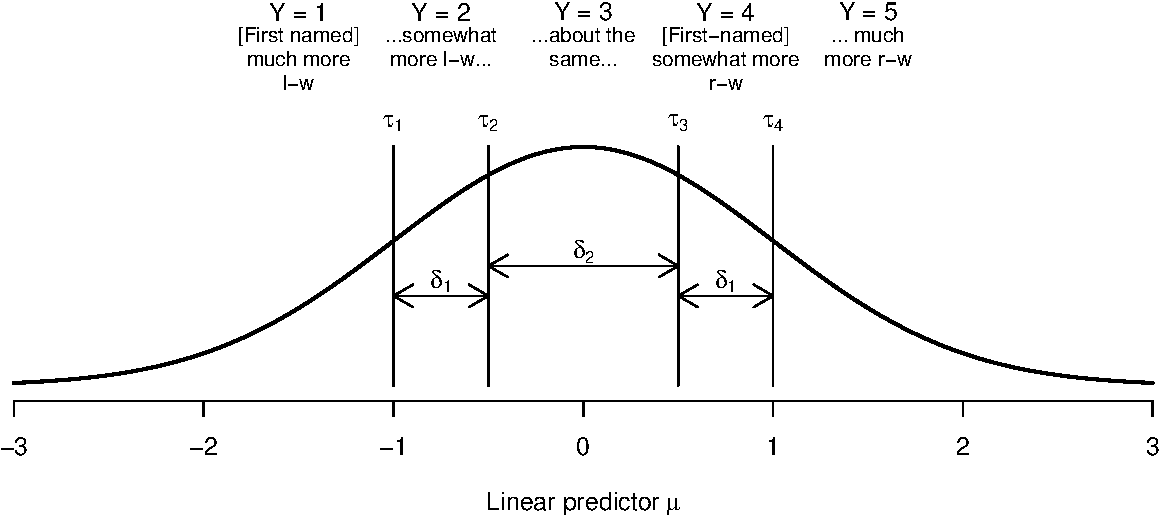
\includegraphics{article_files/figure-pdf/fig-thresh-1.pdf}

}

\caption{\label{fig-thresh}Illustration of the symmetric thresholds
used}

\end{figure}%

The thresholds explain how we can connect the ordered responses given by
councillors to something continuous, but they do not explain where that
continuous variable \(\mu\) comes from. We set up \(\mu\) so that it is
equal to the difference between the latent positions of the two MPs
being compared. We use \(\theta\) to refer to the latent position of
each MP. Referring to \(\theta\) is complicated because the positions of
MPs can be positions of (i) different MPs; (ii) at different times;
(iii) on different dimensions. Additionally, referring to \(\theta\) is
complicated because we sometimes wish to the position of an MP by their
index -- for example, the position of MP number fifty on our list of MPs
-- and sometimes by their role in a comparison -- for example, as the MP
listed as the first-named MP on question forty. Bearing this in mind, we
use subscripts and superscripts so that \(\theta^{Econ.}_{j, t}\) refers
to the position of MP \(j\) on the economic dimension at time \(t\). The
subscript \(j\) runs from 1 to 953 (the number of MPs in our combined
data); the subscript \(t\) is either 1 (referring to the survey
conducted in autum of 2023) or 2 (referring to the survey conducted in
the autumn of 2024). When we write \(\theta^{Cult.}_{A[i], t}\), we
refer to the position on the cultural dimension of the first-named MP in
question \(i\); when we write \(\theta^{Econ.}_{B[i], t}\) we refer to
the position on the economic dimension of the second-named MP in
question \(i\).

With this notation, we can then say that

\doublespacing

\[
\mu_i = \left\{ 
  \begin{array}{ c l }
    \theta^{Econ.}_{B[i], t} - \theta^{Econ.}_{A[i], t} & \quad \textrm{if question was about economics} \\
    \theta^{Cult.}_{B[i], t} - \theta^{Cult.}_{A[i], t} & \quad \textrm{otherwise}
  \end{array}
\right.
\]

\singlespacing

In one sense, this completes the connection between the responses given
by councillors and the positions of the MPs on the two dimensions: we
have specified a model which ends in positions of different MP on two
dimensions at different times. However, this is not the end of the model
specification. Just as with the cutpoints, we chose to introduce certain
elements of structure so that the model makes sense. We chose to capture
three types of structure: temporal, issue, and party.

Consider time first. Even considering just the economic dimension, we've
posited two values of \(\theta\) for each MP -- one value in the first
wave, one value in the second wave. It's very likely that these two
values are close together -- that the distance between the same MP a
year apart is much less than the distance between two MPs chosen at
random but ``measured'' in the same year. We can model this by making
the MP's position at time two equal to their position at time one, plus
a small shift -- or equivalently, we can take the most recent position
as the baseline, and make positions at previous points in time equal to
their most recent position, minus a small shift. Formally,

\[
\theta^{Econ.}_{j, 1} = \theta^{Econ.}_{j, 2} + \nu_j
\]

and

\[
\theta^{Cult.}_{j, 1} = \theta^{Cult.}_{j, 2} + \nu_j
\]

where these small shifts are in turn modelled as coming from a common
distribution with a specified standard deviation.

\[
\nu \sim N(0, 0.1)
\]

By imposing the assumption that the small shifts come from a common
distribution we are able to move back and forth between how large shifts
are on average and how large a shift might be in any particular case.

Now consider party. Just as an MP's position in 2024 is likely to
resemble their position in 2023, so too will the position of a Labour MP
resemble that of another Labour MP much more than it does a Conservative
MP. Although we use the Labour and Conservative parties as examples
here, this applies to any party (or group of MPs who can be treated as
though they were a party). We therefore model each MPs' overall position
as a function of a party-specific component, and a component which is
specific to them. That is,

\doublespacing

\[
\theta^{Econ.}_j = \alpha^{Econ.}_j + \gamma^{Econ.}_{P[j]}
\]

\[
\theta^{Cult.}_j = \alpha^{Cult.}_j + \gamma^{Cult.}_{P[j]}
\]

\singlespacing

where \(P[j]\) gives the party of legislator \(j\), and \(\gamma\)
refers to a set of party-specific fixed effects relative to the
reference party, the Conservatives.

Finally, consider associations between the different dimensions. It is
logically possible that each MPs' position on the economic dimension
tells us nothing about their position about their position on the
cultural dimension -- that a free-marketeer is as likely to be a social
libertarian as they are to be a moralizer. At the same time, there is
lots of evidence to suggest that Western European elites (a category
which necessarily includes members of national legislatures) are very
good at subsuming economic and cultural issues under a single rubric
which has to do with equality. Positions on these two dimensions may
therefore be correlated to a greater or lesser degree. We can
incorporate this into the model by having the idiosyncratic legislator
effects be drawn from a multivariate normal distribution with an
estimated covariance matrix. Formally,

\[
\begin{bmatrix}
\alpha^{Econ.} \\
\alpha^{Cult.}
\end{bmatrix} \sim
N\left(
\begin{bmatrix}
0 \\
0 
\end{bmatrix},
\begin{bmatrix}
\sigma_{Econ.} & \sigma_r \\
\sigma_r & \sigma_{Cult.}
\end{bmatrix}
\right)
\]

The parameters in the model are therefore of three types. There are
parameters of primary interest: the positions of MPs on each dimension
at each time. These are in turn built on parameters of secondary
interest, like the party-specific effects and the legislator-specific
effects on each dimension. Finally, there are ancillary parameters, like
the increments over time, and the variances and covariances. The model
is therefore complicated, but it is only as complicated as it needs to
be to model data asking about two dimensions at two different points in
time.

It would in principle be possible to incorporate other elements into the
model in the same way that party has been incorporated into the model.
Constituency-specific features like the share of the Conservative vote
might be included on the basis that Conservative MPs from an area where
the Conservatives are generally popular are more likely to be right-wing
than Conservative MPs who just eked out a win. However, including these
additional covariates raises further questions (should we expect the
Conservative share of the vote to work in the same way across different
elections?) and complicates attempts to relate MP positions to
characteristics of their area (how can we assess the strength between
voting behaviour in the area and MP positions when voting behaviour in
the area is used to construct the measure of MP positions?).

\subsection{Identifiability and scale}\label{identifiability-and-scale}

Ordinal logit models can suffer from problems of identifiability when
the continuous predictor \(\mu\) is modelled as the difference of two
latent variables, in the sense that different sets of parameter values
can give the same fit to the data. These identifiability issues can be
broken down into issues of scale and location. Problems of scale arise
because we can multiply the latent variables by a constant and divide
the cut-off parameter by that constant, leaving the fit to the data
unchanged. Problems of location arise because we can add on a constant
to all latent variables, leaving the fit to the data unchanged. This is
because the linear predictor depends on the difference between the
latent variables rather than their absolute values.

The issue of scale is dealt with by placing a prior on the first
threshold centred on -2, so that it would no longer be possible to
multiply the latent parameters by some constant and offset that change
by altering the cut-off parameters. The issue of location is dealt with
by the use of the prior on the legislator-specific component of
legislator's ideal points. This prior is centred on zero, and so
solutions would involve adding large positive or negative constants to
the ideal points are penalized.

Although the scale is set by the model (in the sense that the first
cut-off is drawn from a distribution centred on -2 and priors are placed
on the distribution of MP ideal points), this scale is not intuitive. In
this note, we therefore scale MP positions by subtracting the minimum,
dividing by the maximum, and multiplying by 100. This places the
positions on a 0-100 scale. Because the minimum and maximum are
properties of the sample we collected, estimates which are transformed
in this way will not be comparable across different and separately
modelled surveys. Researchers should not therefore interpret these
positions as though they were absolute measurements, or imply that a
score of 25, or 50, or 75, means that an MP is ``left-wing'',
``centrist'', or ``right-wing''.

\subsection{Prior specification}\label{prior-specification}

We place prior distributions on some of these parameters and set some
parameters as fixed. We do this to solve the problems of scale and
location noted above. Specifically, we adopt the following priors for
the cutpoints

\[
\tau_1 \sim N(-2, 0.5)
\]

\[
\delta_1 \sim N^+(0, \sqrt{3})
\]

\[
\delta_2 \sim N^+(0, \sqrt{3})
\]

where \(N^+\) indicates a truncated, or half-normal distribution which
only generates positive values.

We draw party effects from the following common distribution:

\[
\gamma \sim N(0, 4.0)
\]

The most complex priors are the priors placed on the covariance between
legislator specific ideal points. We decompose this covariance matrix
into the product of a scale vector S and a correlation matrix R, where
the prior on the correlation matrix R involves the
Lewandowski-Kurowicka-Joe distribution
(\citeproc{ref-lewandowski2009generating}{Lewandowski, Kurowicka, and
Joe 2009}).

\[
\begin{bmatrix} \sigma_{Econ.} & \sigma_r \\ \sigma_r &
\sigma_{Cult.}  \end{bmatrix} \equiv \operatorname{diag}(S) \cdot R \cdot \operatorname{diag}(S) 
\]

\[
S \equiv
\begin{bmatrix}
\varsigma_{Econ.}, \varsigma_{Cult.}
\end{bmatrix}
\]

\[
\varsigma \sim N^{+}(0, 2);
\]

\[
R \sim LJKCorr(4)
\]

A full justification of these priors is given in the appendix.

\subsection{Estimation}\label{estimation}

The model was estimated in \texttt{rstan}, the R interface to the Stan
programming language {[}Stan Development Team
(\citeproc{ref-rstan}{n.d.}); {]}. The model was set to run for 2,000
iterations, of which 1,000 iterations were discarded as warm-up
iterations. Convergence across the four chains, as measured by the R-hat
statistic, was acceptable.

\section{Results}\label{results}

In this section we describe the results of the analysis, focusing
exclusively on the positions of MPs, rather than any of the secondary
and auxiliary parameters in the model. We make seven broad points
regarding these positions.

\emph{First,} the left-right ordering of parties (according to the
average position of MPs in that party on the economic dimension) makes
sense. Figure~\ref{fig-bees} shows a beeswarm plot of MP's left-right
position on the economic dimension for MPs elected in the 2024 -
parliament. Each plotted point corresponds to the posterior mean. Values
have been rescaled so that the maximum value across all MPs and
iterations is 100, and so that the minimum value is zero. Parties are
ordered by their average (mean) position on this dimension. MPs from
Reform UK are thus the most right-wing party, and the Greens the most
left-wing party. This matches the rank ordering of parties in the 2024
British Election Study Expert Survey, \emph{except that} the expert
survey places Plaid Cymru to the left of the Scottish National Party,
whilst these estimates place the SNP to the left.

Figure~\ref{fig-bees} is valuable not just because it shows the relative
order of parties, but also relative dispersion of the MPs in that party.
When judged by the \emph{range} of MPs positions, the Labour party is
the most variable; when judged by the \emph{standard deviation} of
positions, it is the Conservative party which is most variable. Another
way of saying the same thing is to note that whilst the Labour party has
some outlying MPs to the extreme left and to the centre, many of its MPs
are clustered around the average within the party.

\begin{figure}

\centering{

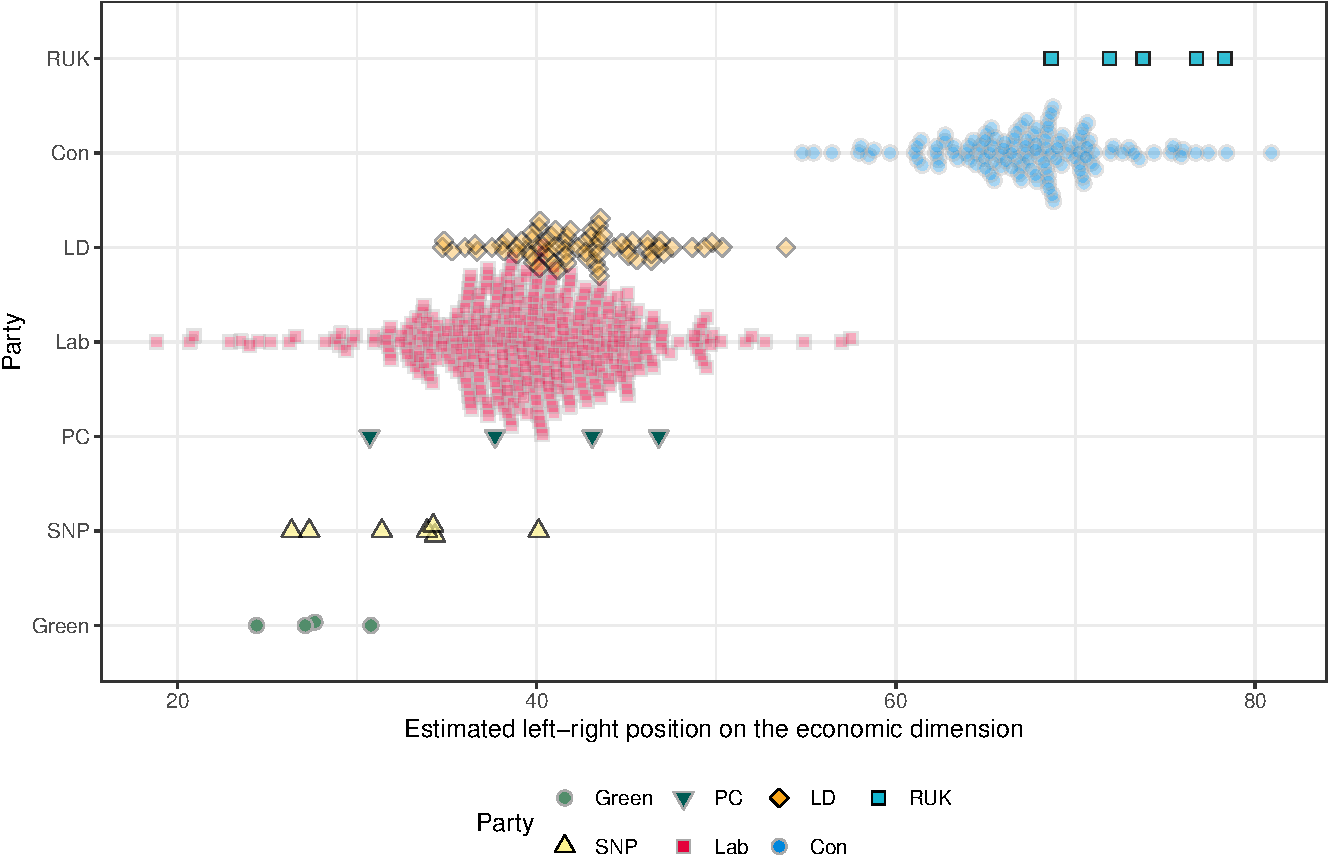
\includegraphics{article_files/figure-pdf/fig-bees-1.pdf}

}

\caption{\label{fig-bees}Bee-swarm plot of MPs' left-right positions on
the economic dimension for MPs elected in 2024.}

\end{figure}%

\emph{Second,} individuals at the extremes of the recovered distribution
are all individuals who we would, on the basis of other evidence,
describe as being at the extreme ends of their party.\footnote{Once
  again, it is important to note that ``extreme'' as used here just
  means ``extreme relative to the other MPs asked about in the survey'',
  and does not imply extremism in an absolute sense.} Whilst
Figure~\ref{fig-bees} is helpful in understand averages, we can gain a
better understanding of these positions by considering individuals MPs
are the left, middle, and right of the distribution.
Table~\ref{tbl-extremes} shows eighteen MPs divided equally between
these three categories. For each MP we show their average position
(column labelled ``Mean'' under ``Position''), the 5th and 95th
percentiles of the distribution (columns marked ``Lo'' and ``Hi'' under
``Position''). We also show equivalent figures for the \emph{rank} of
the MP, where a rank of 1 means that the MP is the most left-wing and a
rank of 614 means that the MP is the most right-wing of the MPs to
feature in the data.

\begin{table}

\caption{\label{tbl-extremes}MPs on the left, middle, and right of the
recovered dimension. Columns Lo and Hi refer to the 2.5th and 97.5th
percentiles of the posterior distribution.}

\centering{

\begin{tabular}[t]{llrrrrrr}
\toprule
\multicolumn{2}{c}{ } & \multicolumn{3}{c}{Position} & \multicolumn{3}{c}{Rank} \\
\cmidrule(l{3pt}r{3pt}){3-5} \cmidrule(l{3pt}r{3pt}){6-8}
MP & Party & Mean & Lo & Hi & Rank & Lo  & Hi \\
\midrule
\addlinespace[0.3em]
\multicolumn{8}{l}{\textbf{Left-wing}}\\
\hspace{1em}Nadia WHITTOME & Lab & 18.8 & 11.6 & 26.2 & 4 & 1 & 14\\
\hspace{1em}Bell RIBEIRO-ADDY & Lab & 20.7 & 15.5 & 25.9 & 5 & 1 & 14\\
\hspace{1em}Diane ABBOTT & Lab & 20.9 & 16.2 & 25.7 & 5 & 1 & 13\\
\hspace{1em}Ian BYRNE & Lab & 22.9 & 17.5 & 28.1 & 9 & 2 & 21\\
\hspace{1em}John MCDONNELL & Lab & 23.5 & 17.3 & 29.7 & 11 & 2 & 31\\
\hspace{1em}Jon TRICKETT & Lab & 24.0 & 17.9 & 30.0 & 12 & 2 & 32\\
\addlinespace[0.3em]
\multicolumn{8}{l}{\textbf{Middle}}\\
\hspace{1em}Warinder JUSS & Lab & 41.4 & 35.1 & 47.9 & 283 & 103 & 440\\
\hspace{1em}Chris VINCE & Lab & 41.5 & 35.3 & 47.7 & 284 & 107 & 440\\
\hspace{1em}Sarah CHAMPION & Lab & 41.5 & 34.8 & 48.0 & 284 & 101 & 441\\
\hspace{1em}James MACCLEARY & LD & 41.6 & 37.0 & 46.2 & 290 & 155 & 411\\
\hspace{1em}Blair MCDOUGALL & Lab & 41.6 & 34.6 & 48.6 & 285 & 94 & 449\\
\hspace{1em}Alex BREWER & LD & 41.6 & 35.6 & 47.4 & 288 & 116 & 434\\
\addlinespace[0.3em]
\multicolumn{8}{l}{\textbf{Right-wing}}\\
\hspace{1em}Priti PATEL & Con & 76.7 & 72.3 & 81.1 & 605 & 590 & 613\\
\hspace{1em}Nigel FARAGE & RUK & 76.7 & 70.6 & 82.9 & 603 & 578 & 614\\
\hspace{1em}Mark FRANCOIS & Con & 77.4 & 73.1 & 81.7 & 607 & 594 & 613\\
\hspace{1em}Rupert LOWE & RUK & 78.3 & 72.3 & 84.3 & 607 & 591 & 614\\
\hspace{1em}Iain DUNCAN SMITH & Con & 78.4 & 72.8 & 84.5 & 608 & 593 & 614\\
\hspace{1em}Suella BRAVERMAN & Con & 80.9 & 76.5 & 85.4 & 612 & 606 & 614\\
\bottomrule
\end{tabular}

}

\end{table}%

The MPs with the furthest left positions are a mix of female MPs from
ethnic minorities and older white men. Nadia Whittome, Bell
Ribeirro-Addy and Diane Abbott all have some possibility of being
\emph{the} most left-wing MP, and we can be confident that they are
amongst the top twenty most left-wing. Ian Byrne, John McDonnell and Jon
Trickett are slightly further to the right, and in their case we could
only confidently say that they were amongst the thirty most left-wing
MPs.

The rank order of these MPs seems \emph{prima facie} plausible. All are
members of the Socialist Campaign Group. Ian Byrne, whilst elected as a
Labour MP, currently sits as an independent, having had the whip
withdrawn after voting to end child benefit caps.

We can be reasonably confident that the individuals at the top of
Table~\ref{tbl-extremes} are to the left of the 2024- parliament, but we
cannot be so confident about the individuals shown in the middle of
Table~\ref{tbl-extremes}. These are individuals who are close to the
middle of the distribution within the Parliament, but who, given the
scale of Labour's victory, need not be ``centrist'' as that term is
commonly understood. The degree of uncertainty for these individuals is
considerable. If we take the newly elected MP for Harlow Chris Vince as
an example -- we can rule out his being amongst the 100 most left-wing
MPs, but can't rule out his being amongst the most right-wing Labour
MPs.

Some degree of certainty returns when we look at individuals furthest to
the right -- two MPs from Reform UK, and four conservatives. Four of
these MPs -- Farage, Lowe, Duncan Smith and Braverman -- have a non-zero
probability of being the most right-wing of MPs to feature in this data;
the other two are not far behind. The positioning of Reform UK MPs is
not surprising, and Braverman has been discussed as a potential
detection to Reform UK following her husband's defection (which took
place after the survey closed, and could therefore not have affected
respondents' evaluation of Braverman).

\begin{figure}

\centering{

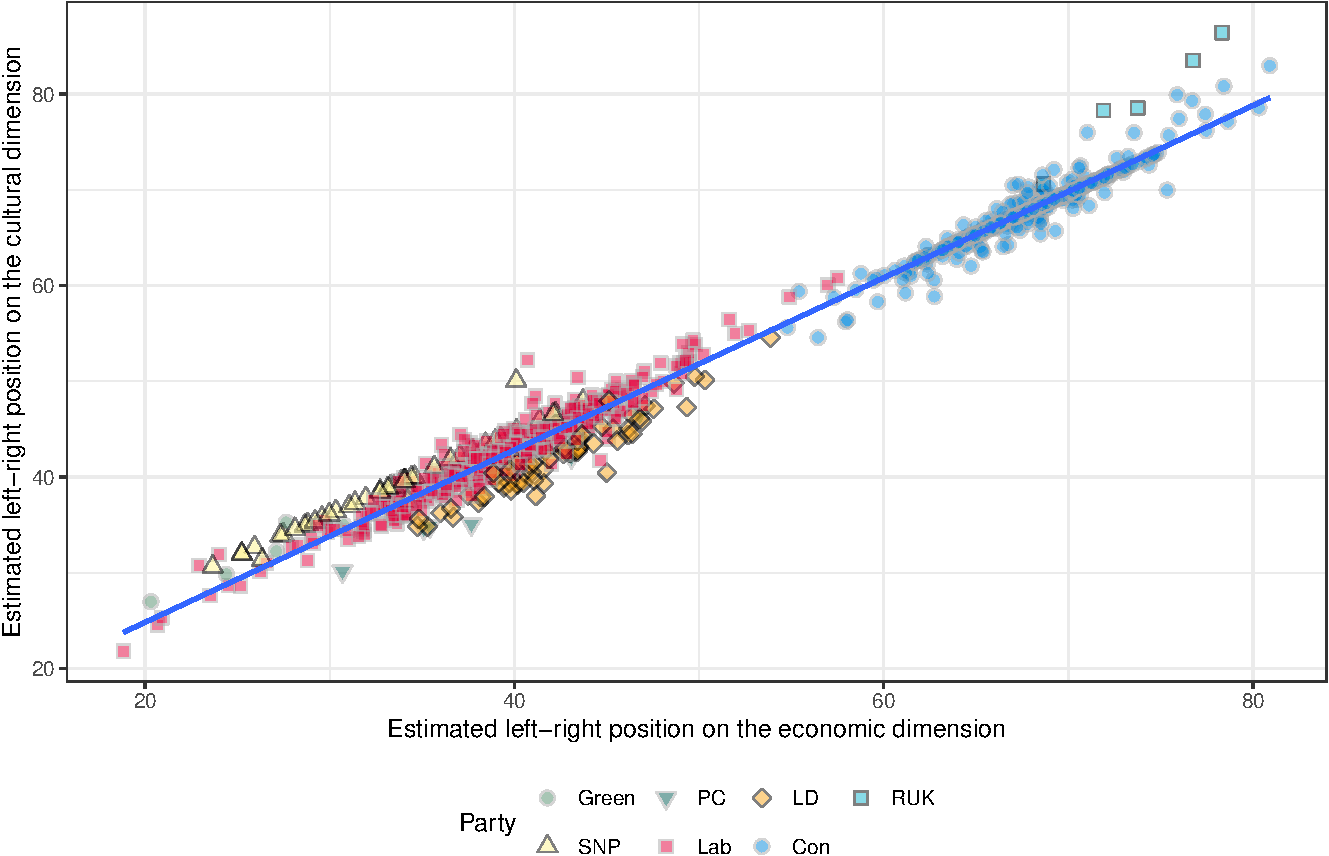
\includegraphics{article_files/figure-pdf/fig-spcult-1.pdf}

}

\caption{\label{fig-spcult}Scatter plot of MPs' left-right positions on
the economic dimension against position on the cultural dimension, for
MPs elected in 2024.}

\end{figure}%

\begin{table}

\caption{\label{tbl-caucus}Average positions and standard deviations of
MPs in different party caucuses, 2019 to 2024 parliament.}

\centering{

\begin{tabular}[t]{lrrr}
\toprule
Group & N & Median & SD\\
\midrule
\addlinespace[0.3em]
\multicolumn{4}{l}{\textbf{Cons.}}\\
\hspace{1em}ERG subscribers & 42 & 69.40 & 3.81\\
\hspace{1em}(All Conservative MPs) & 356 & 68.10 & 3.57\\
\hspace{1em}Tory Reform Group & 13 & 67.45 & 2.95\\
\hspace{1em}One Nation members & 26 & 66.18 & 2.97\\
\addlinespace[0.3em]
\multicolumn{4}{l}{\textbf{Lab.}}\\
\hspace{1em}Tribune Group & 68 & 40.19 & 5.04\\
\hspace{1em}(All Labour MPs) & 191 & 39.21 & 6.09\\
\hspace{1em}Socialist Campaign Group & 34 & 30.42 & 5.79\\
\bottomrule
\end{tabular}

}

\end{table}%

\emph{Third,} the positions of different factions within the two largest
parties (according to the MPs who are members of those factions) make
sense. We have already touched on this in our analysis of the
furthest-left individuals in the Labour Party, all of whom are members
of the Socialist Campaign Group. Table~\ref{tbl-caucus} shows summary
statistics for two Labour factions and three Conservative factions, for
members of the 2019-2024 parliament.\footnote{We use data on the 2019 to
  2024 parliament rather than the 2024 - parliament because new members
  may still be establishing their membership of different party
  factions, and because there are now many fewer surviving members of
  the Tory Reform Group or One Nation.} For Labour, Socialist Campaign
Group MPs are to the left of the party generally, and the party
generally is to the left of Tribune Group MPs. For the Conservatives,
members of the (partially overlapping) Tory Reform and One Nation
groupings are to the left of the party generally, and the party
generally is to the left of European Reform Group subscribers. This
suggests that the estimates are not just correct at the extremes shown
in Table~\ref{tbl-extremes}, but capture differences between relevant
groups of MPs.

\emph{Fourth,} MPs' positions on the economic dimension are almost
identical to their positions on the cultural dimension.
Figure~\ref{fig-bees} and Table~\ref{tbl-extremes} both showed MPs'
positions on the \emph{economic} left-right dimension. Had they instead
showed positions on the cultural left-right dimension, they would not
have been very different. Figure~\ref{fig-spcult} shows the relationship
between MPs' positions on the economic left-right dimension (horizontal
axis) against their positions on the social and cultural dimension
(vertical axis). There is a very strong relationship between positions
on the two dimensions (\(r=\) 0.993). This suggests that MPs' positions
on these two dimensions cannot be distinguished by knowledgeable
observers like councillors. To the extent that there are differences
between positions on these two dimensions, these differences are the
result of party-specific rather than individual-specific differences.
Thus, (most) Reform UK MPs are above and to the left of (most)
Conservative party MPs, indicating that Reform UK MPs are more
right-wing on cultural issues than they are on economic issues.
Conversely, Liberal Democrats are to the bottom and to the right of most
Labour MPs, suggesting that the Liberal Democrats are more right-wing on
economic issues than they are on cultural issues -- or equivalently,
more left-wing on cultural issues than they are on economic issues. The
relative positions of Reform UK and the Liberal Democrats make sense
given the stated ideologies of those parties; it is somewhat harder to
work out why SNP MPs should be judged more socially conservative than
most Labour MPs.

\emph{Fifth,} MPs' positions in 2024 are almost identical to their
positions in 2023. When modelling responses we allowed MP positions to
be correlated across dimensions and connected across waves of the
survey. Having just shown that MPs' positions are near identical across
dimensions of ideology, it should not be surprising to learn that MP
positions are near identical when comparing estimates of positions in
wave 1 and estimates of positions in wave 2. The correlation between the
two positions is almost perfect: \(r=1\) to three decimal places.
Although it is possible that some MPs may shift in position over longer
spans of time, there is no evidence of shifting over this short period
of one year.

\emph{Sixth,} the estimates are strongly associated with other estimates
of MPs' positions. Gaughan (\citeproc{ref-gaughan2024estimating}{2024})
estimates the positions of MPs in the 2019 to 2024 parliament active on
X (formerly Twitter) by performing a latent correspondence analysis on
their follower matrix. The correlation between the estimates here and
those estimates derived from social media is high (\(r=\) 0.936, \(N=\)
558). The correlation between the estimates here and the expert survey
used by Gaughan to validate his estimates is also high (\(r=\) 0.977,
\(N=\) 29) and indeed higher than the correlation between Gaughan's
social media estimates and the expert survey (\(r=\) 0.965, \(N=\) 29).

An earlier set of estimates comes from Hanretty, Lauderdale, and Vivyan
(\citeproc{ref-hanretty2017dyadic}{2017}) who (following Kellermann
(\citeproc{ref-kellermann2012estimating}{2012})) estimate the positions
of backbenchers in the 2010-2015 parliament by analysing the early day
motions they sign. The correlation with these estimates is also
extremely high (\(r=\) 0.923, \(N=\) 175).

There is therefore evidence from other attempts to estimate MPs'
positions to suggest that the estimates presented here display
convergent validity. We argue that our estimates are preferable to these
other estimates because of their greater coverage, and because they
display a stronger association with expert placements, which are as
close as we will get to ``ground truth''.

\begin{figure}

\centering{

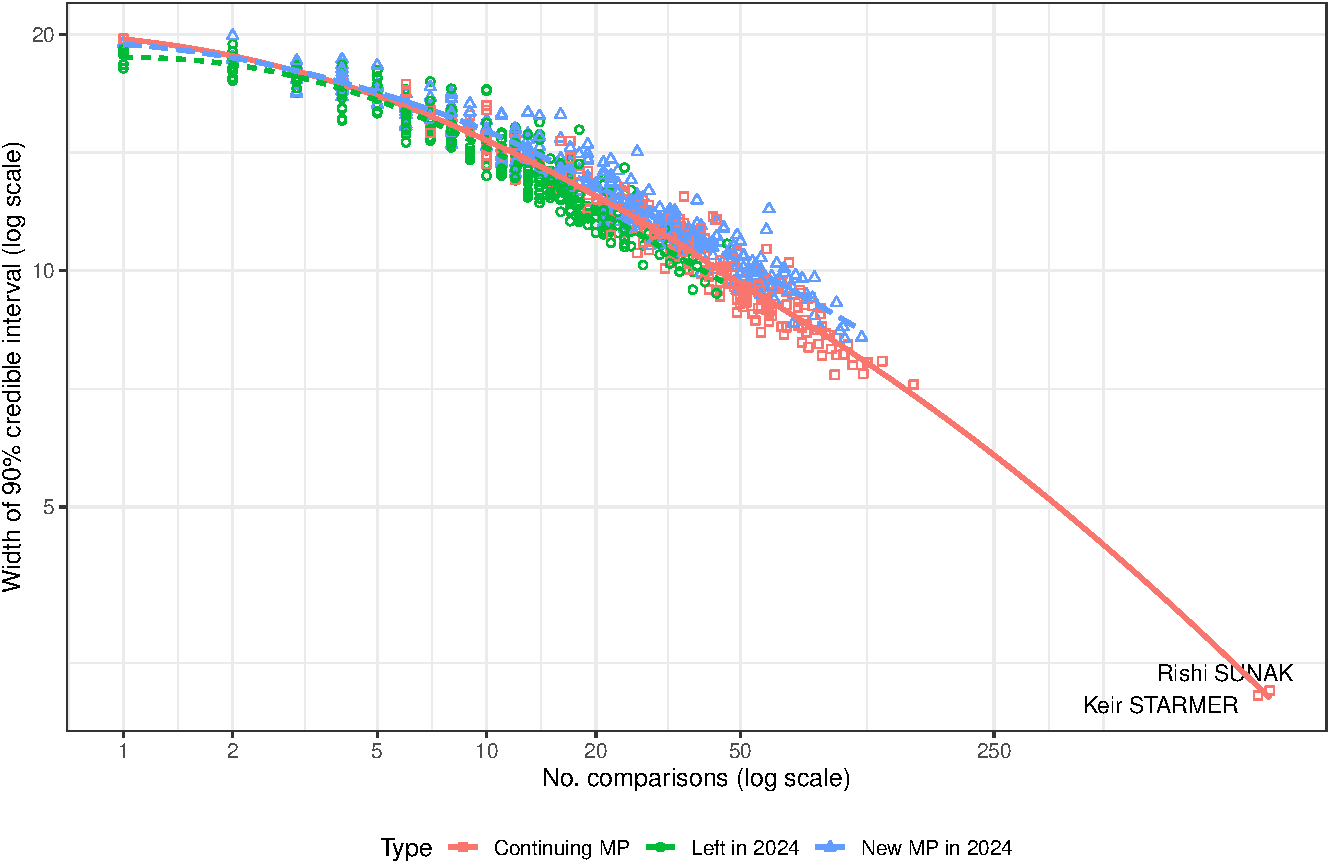
\includegraphics{article_files/figure-pdf/fig-uncertainty-1.pdf}

}

\caption{\label{fig-uncertainty}Uncertainty in estimates as a function
of the number of comparisons}

\end{figure}%

\emph{Seventh,} uncertainty in the position of MPs is primarily a
function of the number of times they were asked about and secondarily a
function of whether they are new MPs. Figure~\ref{fig-uncertainty} shows
the width of the 90\% credible interval (logged, on the vertical axis)
as a function of the number of comparisons (logged, on the horizontal
scale). The three trend lines show nonlinear smooths for three groups of
MPs: MPs who continued between both parliaments, MPs who left
(voluntarily or otherwise) at the end of the 2019-2024 parliament, and
MPs elected in the 2024 parliament but who did not sit in the 2019-2024
parliament. Although difficult to see on the graph, the trend line for
``new'' entrants ixs almost always higher than the trend line for the
other two types of MPs.

\section{Conclusion}\label{conclusion}

In this note we have described a method that we use for inferring the
left-right positions of MPs from a survey of local councillors. This
method, applied to this data, means that we can provide estimates of
positions for almost all MPs, estimates which are informed by local
knowledge and which come with estimates of uncertainty. These estimates
will be useful for researchers who are interested in MPs' positions as
an outcome (of, variously, initial selection, subsequent re-election,
and possible de-selection) and MPs' positions as predictors of other
outcomes (for example: cabinet recruitment and declarations of support
in leadership contests).

We believe that these estimates of MP positions are superior to other
existing estimates of MP positions. Estimates of MP positions based on
co-sponsorship of early day motions are possible only for backbench MPs,
and suffer from the problem that many fewer MPs now sign early day
motions. Estimates from social media are only available for those MPs
who are active on a specific social media platform, and exhibit lower
correlation with expert placements of MPs.

This method is not perfect. It cannot be applied retrospectively and
like any survey-based research it costs money. In addition when applied
to a single parliamentary term -- particularly a parliamentary term
where there are a large number of new MPs -- the degree of uncertainty
may be very large indeed, such that we cannot discriminate between the
positions of most new entrants. When applied to a single parliamentary
term, there are also issues with regional isolates -- areas where most
MPs are uniformly to the left or right of the anchor MPs, and where
other MPs appear as very left- or right-wing as a result. This issue
arises in Scotland, where many MPs are to the left of both Keir Starmer
and Rishi Sunak, and where Liberal Democrat and Conservative MPs appear
very right-wing as a result, and in Essex, where many MPs are to the
right of both Keir Starmer and Rishi Sunak, and where other MPs,
including some Conservative MPs, can appear more left-wing than they may
in fact be.

We have motivated this note on the basis that these estimates can be
\emph{useful}. Whilst contributing useful data is important (and worthy
of publication) we also think that our survey suggests some substantive
conclusions. Specifically, it suggests that MPs' positions on the
economic and sociocultural dimensions are so highly correlated that
knowledgeable observers position the average MP in the same place on
both dimensions. This does not imply that for any specific MP their
positions on those dimensions are identical. For any high profile MP
with a large public record, it is possible that knowledgeable observers
might be able to identify different positions on both those domains.
These individuals are, by definition, not average. More generally, for
any MP it is possible that the MP does \emph{in fact} have different
positions on these dimensions, but that they have not said or done
enough which would lead a knowledgeable observer to identify these
contrasting positions correctly. As always, we can only infer positions
or ideal points from what MPs do or say; no social science method is
capable of peering into their soul.

\section*{References}\label{references}
\addcontentsline{toc}{section}{References}

\phantomsection\label{refs}
\begin{CSLReferences}{1}{0}
\bibitem[\citeproctext]{ref-breunig2021measuring}
Breunig, C, B Guinaudeau, and S Roth. 2021. {``Measuring Legislators'
Ideological Position Using Pairwise-Comparisons.''} Working paper.

\bibitem[\citeproctext]{ref-burkner2019ordinal}
Bürkner, Paul-Christian, and Matti Vuorre. 2019. {``Ordinal Regression
Models in Psychology: A Tutorial.''} \emph{Advances in Methods and
Practices in Psychological Science} 2 (1): 77--101.

\bibitem[\citeproctext]{ref-catalinac2018positioning}
Catalinac, Amy. 2018. {``Positioning Under Alternative Electoral
Systems: Evidence from {J}apanese Candidate Election Manifestos.''}
\emph{American Political Science Review} 112 (1): 31--48.

\bibitem[\citeproctext]{ref-christensen2019clm}
Christensen, Rune Haubo B. 2019.
\url{https://cran.r-project.org/web/packages/ordinal/vignettes/clm_article.pdf}.

\bibitem[\citeproctext]{ref-gaughan2024estimating}
Gaughan, Conor. 2024. {``Estimating Ideal Points of British MPs Through
Their Social Media Followership.''} \emph{British Journal of Political
Science}, 1--13.

\bibitem[\citeproctext]{ref-hanretty2017dyadic}
Hanretty, Chris, Benjamin E Lauderdale, and Nick Vivyan. 2017. {``Dyadic
Representation in a {W}estminster System.''} \emph{Legislative Studies
Quarterly} 42 (2): 235--67.

\bibitem[\citeproctext]{ref-heppell2013cameron}
Heppell, Timothy. 2013. {``Cameron and Liberal Conservatism: Attitudes
Within the Parliamentary {C}onservative Party and {C}onservative
Ministers.''} \emph{The British Journal of Politics and International
Relations} 15 (3): 340--61.

\bibitem[\citeproctext]{ref-hopkins2022trump}
Hopkins, Daniel J, and Hans Noel. 2022. {``Trump and the Shifting
Meaning of {`Conservative'}: Using Activists' Pairwise Comparisons to
Measure Politicians' Perceived Ideologies.''} \emph{American Political
Science Review} 116 (3): 1133--40.

\bibitem[\citeproctext]{ref-johnson2003use}
Johnson, Timothy R. 2003. {``On the Use of Heterogeneous Thresholds
Ordinal Regression Models to Account for Individual Differences in
Response Style.''} \emph{Psychometrika} 68: 563--83.

\bibitem[\citeproctext]{ref-kellermann2012estimating}
Kellermann, Michael. 2012. {``Estimating Ideal Points in the {B}ritish
{H}ouse of {C}ommons Using Early Day Motions.''} \emph{American Journal
of Political Science} 56 (3): 757--71.

\bibitem[\citeproctext]{ref-lauderdale2016measuring}
Lauderdale, Benjamin E, and Alexander Herzog. 2016. {``Measuring
Political Positions from Legislative Speech.''} \emph{Political
Analysis} 24 (3): 374--94.

\bibitem[\citeproctext]{ref-lewandowski2009generating}
Lewandowski, Daniel, Dorota Kurowicka, and Harry Joe. 2009.
{``Generating Random Correlation Matrices Based on Vines and Extended
Onion Method.''} \emph{Journal of Multivariate Analysis} 100 (9):
1989--2001.

\bibitem[\citeproctext]{ref-o2022transformation}
O'Grady, Tom. 2022. \emph{The Transformation of {B}ritish Welfare
Policy: Politics, Discourse, and Public Opinion}. Oxford University
Press.

\bibitem[\citeproctext]{ref-spirling2007uk}
Spirling, Arthur, and Iain McLean. 2007. {``{UK OC OK}? Interpreting
Optimal Classification Scores for the {UK} {H}ouse of {C}ommons.''}
\emph{Political Analysis} 15 (1): 85--96.

\bibitem[\citeproctext]{ref-rstan}
Stan Development Team. n.d. {``{RStan}: The {R} Interface to {Stan}.''}
\url{https://mc-stan.org/}.

\bibitem[\citeproctext]{ref-volkens2013mapping}
Volkens, Andrea, Judith Bara, Ian Budge, Michael D McDonald, and
Hans-Dieter Klingemann. 2013. \emph{Mapping Policy Preferences from
Texts: Statistical Solutions for Manifesto Analysts}. Vol. 3. OUP
Oxford.

\end{CSLReferences}




\end{document}
